In this work, we envision a sophisticated, end-to-end toolchain that supports not only construction but also the verification of the engineering artifacts (including software) for high-confidence applications. The development flow provided by the toolchain shall follow a variation of the classical V-model (with software and hardware development on the two branches), with some refinements added at the various stages. Figure \ref{fig:toolchain} illustrates this development flow.

\begin{figure}[h]

   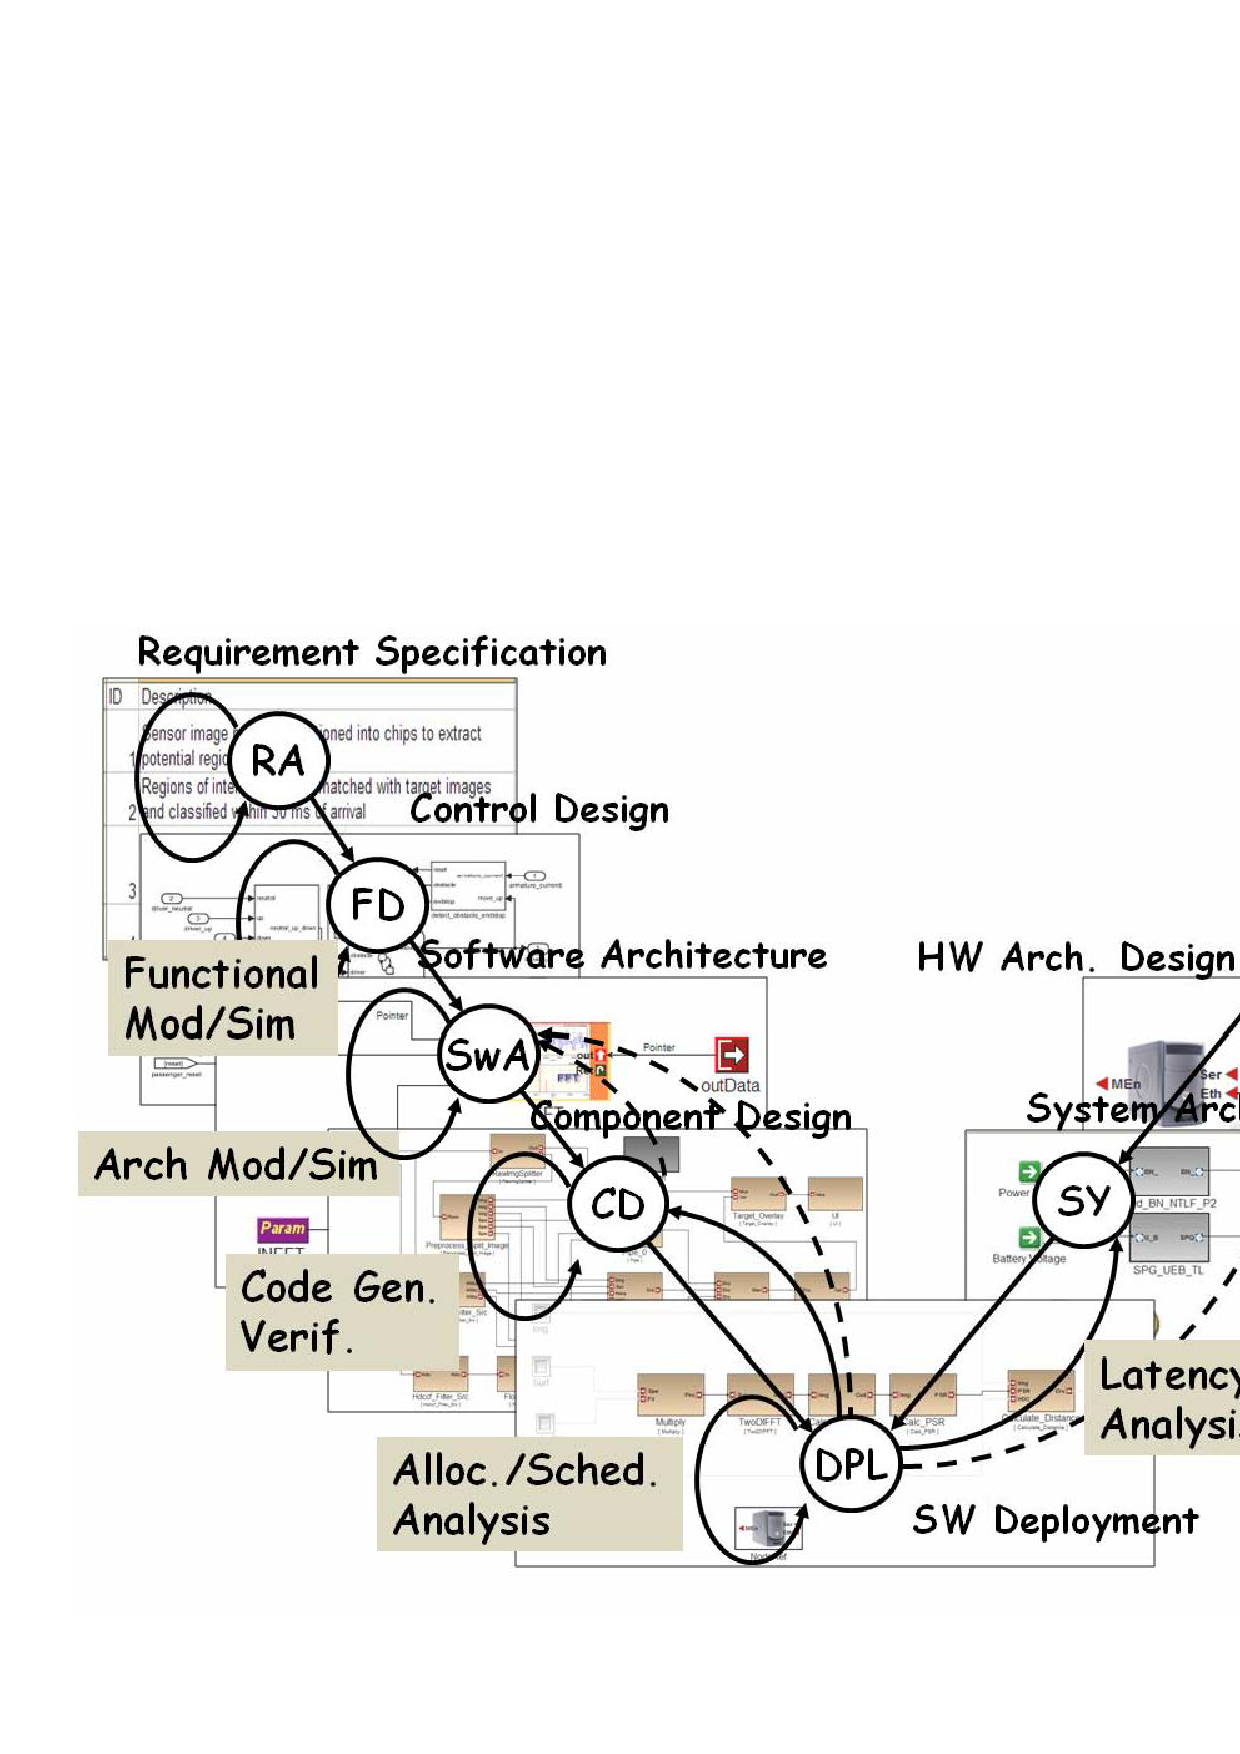
\includegraphics[width=0.9\columnwidth]{toolchain}
   \caption{Conceptual model of the toolchain: Development flow}
   \label{fig:toolchain}
\end{figure}

In the development process, requirements analysis (RA) is followed by functional design (FD) of the controllers, typically enacted using a controller modeling tool like Simulink/Stateflow or Matrix-X. Controller models typically include (synchronous) dataflow (block) diagrams and some variant of Statechart \cite{harel:statecharts} models. This step is followed by laying out the overall software architecture (SwA) as well as the hardware architecture (HwA) (on the other side). We assume that models that capture both the SwA and HwA aspects of the system are available or producible. Controllers (in the form of models) are componentized in the component design (CD) phase - this usually involves 'wrapping' the code generated from the block diagrams such that they become integratable components on some run-time component framework. On the hardware side, the architecture design is consists of (1) system architecture (SY) design (integration of hardware and software aspects), and (2) how software components must be deployed on hardware elements (DPL). We envision that multiple, yet interlinked models will be used in all stages of the design process, and engineers work through the design flow via models to construct the system.

We also envision that such a model-based design flow integrates a number of verification activities. For instance, in FD today we often use simulation for verifying the functionality of the controllers. In the future this could be extended with the use of advanced model checking tools. When code is generated from the models, the generated code could be subjected to code-level verification regimes to check, for example, that the generated code will work with a bounded stack. When components are allocated to hardware and software resources (e.g. 'tasks'), the resulting system model could be used for schedulability analysis (assuming the problem is decidable and data for worst-case execution time is available).

In summary, we envision that model-based embedded software development toolchains will be extended with verification and validation tools such that models and code could be continuously subjected to these checks, and the results could be used in the certification of the embedded systems produced. Below we discuss some design rationales for the actual implementation of the toolchain.

\SubSection{Platform}
In order to reduce design complexity, we believe a toolchain needs to follow the principles of platform-based design \cite{alberto:2002}.  A 'platform' in this case means a 'component framework' that provides some common services used by all applications. Existing commercial real-time operating systems typically provide elementary services (concurrent tasks, task synchronization and communication, partitioning, etc.). We believe embedded systems require better software platforms with higher-level services, e.g. remote method invocation, time-triggered execution, support for composing systems from components, fault-tolerant real-time communication, replica determinism, and others. The main expected feature of a component framework is to be able to construct systems from components in such a way that the properties of the system  could be determined from the properties of the components and the way they are composed. However, this composability property is tightly interwoven with the provided services of the framework, i.e. they cannot be separated.

Component frameworks for embedded systems are an active area of research, and there are numerous research prototypes as well as industrial implementations. High-confidence systems require platforms that provide services and guarantees for needed properties, e.g. fault containment, temporal firewalls, etc. These critical services (like partitioning) should be provided by the platform and not re-implemented from scratch by system developers.

Note that the platform, as a component framework, also defines a 'Model of Computation' \cite{Lee:M97/11}. An MoC governs how the concurrent objects of an application interact, how synchronization and communication takes place, and how these activities unfold in time. The MoC also determines how composition works and, implicitly, how the system-level properties could be derived from the component level properties and the composition operation.

The above discussion underlines the need for the careful selection of a platform. Initially in our work, we wanted to focus on the design of digital controllers that operate periodically, i.e. according to precise timing specifications. These controller components could communicate with other controller components as well as software components that encapsulate peripheral interfaces. For high-confidence designs, distributed fault-tolerance (while maintaining real-time properties) is essential, and, according to our knowledge, currently there is one truly industrial strength approach that provides all of these: the Time-Triggered Architecture (TTA) \cite{kopetz:2001-22}. Hence, in the initial version of the toolchain, our chosen platform was the TTA.

\SubSection{Modeling language}
Model-driven development is based on the use of models expressed in modeling languages, while model-integrated computing refines this paradigm by emphasizing the use of \emph{domain-specific} modeling languages. UML, in its default form, is capable of expressing domain-specificity through the use of UML profiles; however, we did not find profiles adequate for our applications. Hence, we have chosen to develop a domain-specific language for modeling and deploying high-confidence control systems.

A modeling language to support the development flow described above should have several desired properties: (1) it should be able to ``understand'' (and import) functional models from existing design tools, (2) it should be able to capture the relevant aspects of the system architecture and hardware, (3) it should support the modeling of components and the componentization of functional models, and (4) it should be able to model the deployment of the software architecture onto the hardware architecture. The need for being able to import existing models from functional modeling tools is not a deeply justified requirement, it is merely pragmatic.

The design of the language was influenced by two factors: (1) the MoC implemented by the platform and (2) the need for integration with legacy modeling and embedded systems tools. We have chosen Simulink/Stateflow as the supported ``legacy'' tool. As our chosen MoC relies on periodically scheduled, time-triggered components, it was natural to use this concept as the basis for our modeling language and interpret the imported Simulink blocks as the implementation of these components. Communication links (signals) between Simulink blocks are mapped onto TTA messages passed between the tasks. The resulting language provides a componentized view of (discrete-time) Simulink models that are scheduled periodically (with a fixed rate) and communicate with each other using time-triggered messages.

Note that this is only the initial implementation of the modeling language, and we plan to extend it towards other MoC-s. For instance, we need provisions for event-triggered communication and components. Such event-triggered component structures give rise to interesting communication patterns that seem to be very useful in practical systems (e.g. publish-subscribe, rendezvous, and broadcast). We are planning to integrate support for these in our modeling language in the near future.

\SubSection{Code generators and synthesis tools}
Model-based development is often called higher-level programming, i.e. programming using models instead of an algorithmic language. This means that we need to generate executable code from the models. This also means that the generator could be more than just a simple model-to-code translator; it could be a code 'synthesizer' that synthesizes low-level code from higher-level specifications. Synthesis is different from translation as it can involve some notion of search during the code generation process. For instance, if scaled fixed-point arithmetic is to be used, the synthesizer could automatically select the appropriate scaling factors for every operational step (in, say, a dataflow model) based on the value ranges for the input and output variables and the number of bits available for representing fixed-point numbers on the hardware.

Generating code from dataflow and Statechart models is a well-defined and solved problem, and there are many actual implementations. Code synthesis from higher-level models, however, is an active area of research with many open questions regarding code efficiency and correctness.

In our toolchain we created a number of code generators (no synthesizers yet). In the construction of the two main code generators (one for Simulink-style models and another one for Stateflow-style models), we have used a higher-level approach based on graph transformations \cite{isis:great}. This approach is based on the assumption that (1) models are typed and attributed graphs with some specific structure (governed by the metamodel of the modeling language) and (2) the executable code can be produced in the form of an abstract syntax graph (which is then printed directly into source code). This graph transformation-based approach allows a higher-level representation of the translation process, which lends itself to algorithmic analysis of the transformations.

\SubSection{Verification and analysis}
As discussed above, verification and analysis must be an inseparable part of the development process for high-confidence systems. There are a number of well-known verification techniques and tools; however, we must emphasize two points of concern here: (1) the verification tools often operate on the models (i.e. an abstraction of the system), not the code of the system and (2) verification results are meaningful only if the model transformations (that map design models into analysis models or into code) are correct, i.e. properties are carried over by the transformation and the transformation does not add any new artifacts that extend the behavior of the generated code compared to that of the model.

As we envision it, there are several opportunities and challenges for verification. First, verification can be done directly on the design models; in this case the design language and the analysis language are one and the same. Unfortunately, this is not a common case except in simulation-based approaches. Second, verification can be done on analysis models (i.e. design models re-expressed in the language of some verification tool), but it must be shown that the transformation of design models into analysis models is correct, i.e. the analysis results hold for the original models. Third, verification can be done on the level of the (generated) code, but we typically lose the higher-level abstractions of the original models that could make reasoning more efficient. In the first two cases we also need to address the question of how the verification results carry forward to the (executable) code such that we can claim that the code (the final product that runs on an embedded system) satisfies properties of interest.

Construction of such verification-based tools and the verifying of model translators is an active area of research. The correctness of a model transformation is a very complex problem, but some early results indicate a promising direction \cite{ananth:2006}: instead of proving the correctness of a transformation in general, one can show that a particular instance of a transformation preserves the properties of interest and, thus, conclude that the properties hold for the input of the transformation as well.

Another promising direction that we plan to pursue later with our toolchain is a connection between the models and the generated code. We are working on extending the code generator such that it carries forward model-level information to the generated code (in the form of annotations) that provide help for the code-level verifier to check model-level properties on the code. This connection could potentially be used to improve performance, as the verifier could reason using higher-level abstractions than those immediately available from the code.

